\documentclass[nooutcomes,noauthor,handout,12pt]{ximera}

\graphicspath{  
{./}
{./whoAreYou/}
{./drawingWithTheTurtle/}
{./bisectionMethod/}
{./circles/}
{./anglesAndRightTriangles/}
{./lawOfSines/}
{./lawOfCosines/}
{./plotter/}
{./staircases/}
{./pitch/}
{./qualityControl/}
{./symmetry/}
{./nGonBlock/}
}


%% page layout
\usepackage[cm,headings]{fullpage}
\raggedright
\setlength\headheight{13.6pt}


%% fonts
\usepackage{euler}

\usepackage{FiraMono}
\renewcommand\familydefault{\ttdefault} 
\usepackage[defaultmathsizes]{mathastext}
\usepackage[htt]{hyphenat}

\usepackage[T1]{fontenc}
\usepackage[scaled=1]{FiraSans}

%\usepackage{wedn}
\usepackage{pbsi} %% Answer font


\usepackage{cancel} %% strike through in pitch/pitch.tex


%% \usepackage{ulem} %% 
%% \renewcommand{\ULthickness}{2pt}% changes underline thickness

\tikzset{>=stealth}

\usepackage{adjustbox}

\setcounter{titlenumber}{-1}

%% journal style
\makeatletter
\newcommand\journalstyle{%
  \def\activitystyle{activity-chapter}
  \def\maketitle{%
    \addtocounter{titlenumber}{1}%
                {\flushleft\small\sffamily\bfseries\@pretitle\par\vspace{-1.5em}}%
                {\flushleft\LARGE\sffamily\bfseries\thetitlenumber\hspace{1em}\@title \par }%
                {\vskip .6em\noindent\textit\theabstract\setcounter{question}{0}\setcounter{sectiontitlenumber}{0}}%
                    \par\vspace{2em}
                    \phantomsection\addcontentsline{toc}{section}{\thetitlenumber\hspace{1em}\textbf{\@title}}%
                     }}
\makeatother



%% thm like environments
\let\question\relax
\let\endquestion\relax

\newtheoremstyle{QuestionStyle}{\topsep}{\topsep}%%% space between body and thm
		{}                      %%% Thm body font
		{}                              %%% Indent amount (empty = no indent)
		{\bfseries}            %%% Thm head font
		{)}                              %%% Punctuation after thm head
		{ }                           %%% Space after thm head
		{\thmnumber{#2}\thmnote{ \bfseries(#3)}}%%% Thm head spec
\theoremstyle{QuestionStyle}
\newtheorem{question}{}



\let\freeResponse\relax
\let\endfreeResponse\relax

%% \newtheoremstyle{ResponseStyle}{\topsep}{\topsep}%%% space between body and thm
%% 		{\wedn\bfseries}                      %%% Thm body font
%% 		{}                              %%% Indent amount (empty = no indent)
%% 		{\wedn\bfseries}            %%% Thm head font
%% 		{}                              %%% Punctuation after thm head
%% 		{3ex}                           %%% Space after thm head
%% 		{\underline{\underline{\thmname{#1}}}}%%% Thm head spec
%% \theoremstyle{ResponseStyle}

\usepackage[tikz]{mdframed}
\mdfdefinestyle{ResponseStyle}{leftmargin=1cm,linecolor=black,roundcorner=5pt,
, font=\bsifamily,}%font=\wedn\bfseries\upshape,}


\ifhandout
\NewEnviron{freeResponse}{}
\else
%\newtheorem{freeResponse}{Response:}
\newenvironment{freeResponse}{\begin{mdframed}[style=ResponseStyle]}{\end{mdframed}}
\fi



%% attempting to automate outcomes.

%% \newwrite\outcomefile
%%   \immediate\openout\outcomefile=\jobname.oc
%% \renewcommand{\outcome}[1]{\edef\theoutcomes{\theoutcomes #1~}%
%% \immediate\write\outcomefile{\unexpanded{\outcome}{#1}}}

%% \newcommand{\outcomelist}{\begin{itemize}\theoutcomes\end{itemize}}

%% \NewEnviron{listOutcomes}{\small\sffamily
%% After answering the following questions, students should be able to:
%% \begin{itemize}
%% \BODY
%% \end{itemize}
%% }
\usepackage[tikz]{mdframed}
\mdfdefinestyle{OutcomeStyle}{leftmargin=2cm,rightmargin=2cm,linecolor=black,roundcorner=5pt,
, font=\small\sffamily,}%font=\wedn\bfseries\upshape,}
\newenvironment{listOutcomes}{\begin{mdframed}[style=OutcomeStyle]After answering the following questions, students should be able to:\begin{itemize}}{\end{itemize}\end{mdframed}}



%% my commands

\newcommand{\snap}{{\bfseries\itshape\textsf{Snap!}}}
\newcommand{\flavor}{\link[\snap]{https://snap.berkeley.edu/}}
\newcommand{\mooculus}{\textsf{\textbf{MOOC}\textnormal{\textsf{ULUS}}}}


\usepackage{tkz-euclide}
\tikzstyle geometryDiagrams=[rounded corners=.5pt,ultra thick,color=black]
\colorlet{penColor}{black} % Color of a curve in a plot



\ifhandout\newcommand{\mynewpage}{\newpage}\else\newcommand{\mynewpage}{}\fi

\title{Quick questions}

\author{Bart Snapp}

\begin{document}
\begin{abstract}
  Let's apply our knowledge.
\end{abstract}
\maketitle


\begin{listOutcomes}
\item Work with percent increase and percent decrease.
\item Apply the relation between linear scaling and area scaling.
\item Apply the relation between linear scaling and volume scaling.
\item Translate classroom mathematics into real world mathematics. 
\end{listOutcomes}
  %Toybox, cereal box, Lego box? Estimate a discrete unit? 

\mynewpage


\begin{question}
  You are planning a building with a square parking lot.
  \begin{enumerate}
  \item You realize that if you re-arrange your design, you can make
    the square parking lot $13\%$ bigger on each side. How many more
    cars can park in this new lot? Answer in terms of a percent and
    explain your reasoning.
  \item Upon further inspection, you realize that with just a little
    more re-arrangement, you can turn your original square parking lot
    into a rectangle that is $9\%$ larger on one side, and $22\%$
    larger on the other. How many more cars can park in this new lot?
    Answer in terms of a percent and explain your reasoning.
  \end{enumerate}
  \begin{freeResponse}
    \begin{enumerate}
    \item Well, if the side length is $13\%$ bigger, then the area is
      \[
      1.13\cdot 1.13 = \text{$28$ percent larger}
      \]
      so, we could park $28\%$ more cars.
    \item So if we make a rectangle parking lot that is $9\%$ larger on
      one side, and $22\%$ larger on the other, then the area is
      \[
      1.09\cdot 1.22 = \text{$33$ percent larger}
      \]
      so, we could park $33\%$ more cars.
    \end{enumerate}
  \end{freeResponse}
\end{question}
\mynewpage

\begin{question}
  You decide to buy an inflatable pool that is $10$ feet wide and $3$
  feet deep:
  \begin{center}
    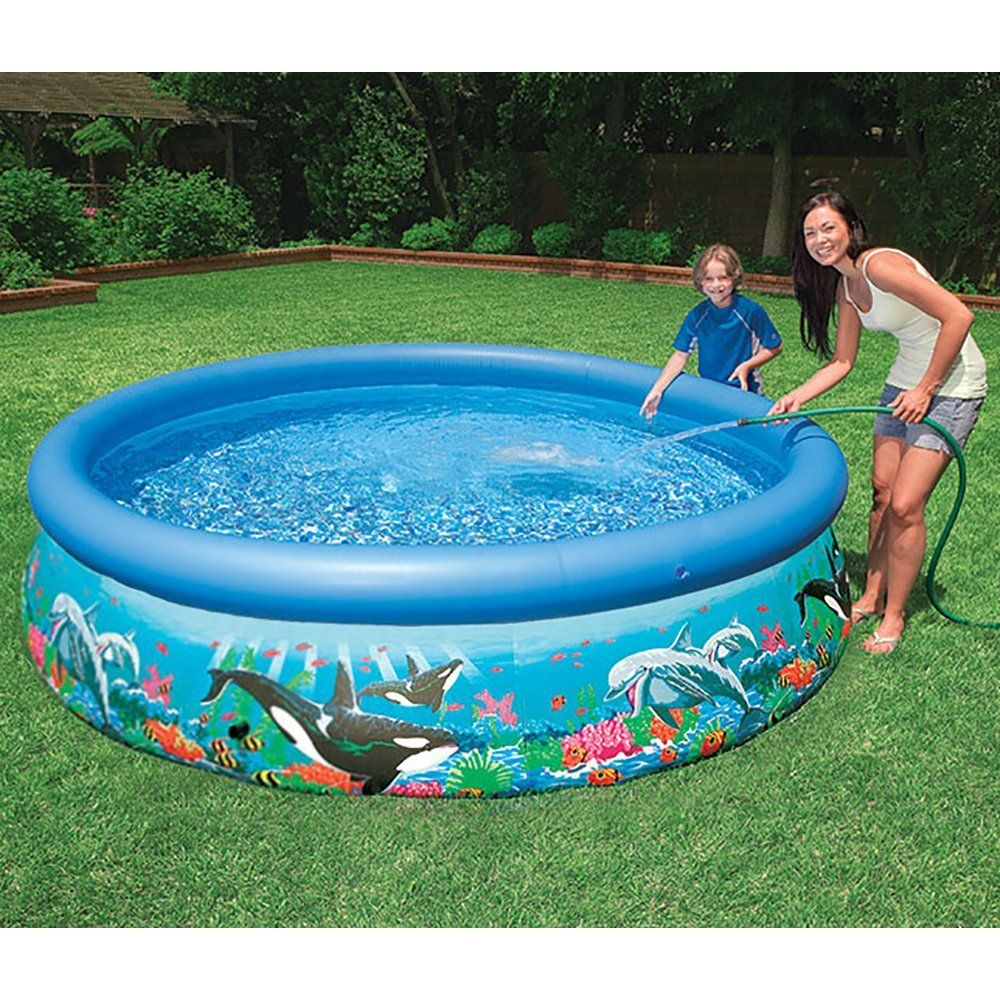
\includegraphics[width=.4\textwidth]{tenFtPool.jpg}
  \end{center}
  \begin{enumerate}
    \item Suppose you have a coupon for $10\%$ off the price of the
      pool above. At the checkout counter, the cashier asks you, ``Do
      you want me to compute the discount before or after the tax?''
      \textbf{To save the most money, should you compute the discount
        before or after tax?} Explain your reasoning.
    \item Now that you have the pool, you plan to have a pool party at
      $4$pm the next day. Given that you can fill a bowl that is $5$
      inches wide and $1.5$ inches deep with water in just $1/4$th of
      a second, \textbf{when should you start filling your pool to
        ensure it is ready by $\boldsymbol 4$pm?}.  Respect significant digits and explain your reasoning.
  \end{enumerate}
  \begin{freeResponse}
    \begin{enumerate}
    \item Well, it doesn't matter, because multiplication is commutative.
      \[
      0.9 \cdot (\text{tax}) \cdot (\text{cost of pool})= (\text{tax})\cdot
      0.9\cdot (\text{cost of pool}).
      \]
    \item So, the pool has
      \[
      12^3 \cdot 2^3 = 13824
      \]
      times as much volume as the bowl of water. Hence it will take
      \[
      13824/4 = 3456 ~\text{seconds}
      \]
      or
      \[
      \frac{3456}{60\cdot 60} \approx 1~\text{hour}.
      \]
      We should start filling the pool at $3$pm to be ready by $4$pm.
    \end{enumerate}
  \end{freeResponse}
\end{question}
\mynewpage




\begin{question} 
  You've designed a roughly spherical water tank:
\begin{center}%http://classes.dma.ucla.edu/Spring16/154/wp-content/uploads/2016/04/RMendez_Photo_1950s.pdf
  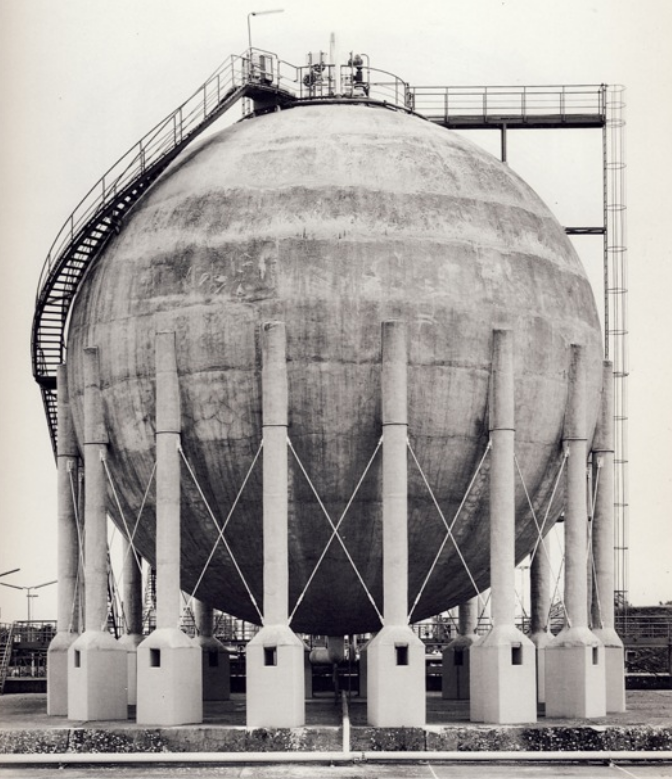
\includegraphics[width=.4\textwidth]{tank.png}  
\end{center}
\begin{enumerate}
\item How does the cost of the raw materials will change if the radius
  is reduced by $10\%$?
\item How does the capacity change if the radius is reduced by $10\%$?
\item How does the filled-weight change if the radius is increased by
  $10\%$?
\item How does the empty-weight change if the radius is increased by
  $10\%$.
\item How does the filled-weight change if the empty-weight is
  increased by $10\%$.
\end{enumerate}
\textbf{In each case, answer in terms of a percent and EXPLAIN your reasoning.}
\begin{freeResponse}
  \begin{enumerate}
  \item Well, the amount of raw materials (and hence the cost) scales
    like the surface area. So if the radius is reduced by $10\%$, the
    cost of the raw materials is reduced by
    \[
    0.9\cdot 0.9 = 0.81
    \]
    and hence is reduced by $19\%$.
  \item The capacity scales like the volume.  So if the radius is
    reduced by $10\%$, the capacity is reduced by
    \[
    0.9\cdot 0.9\cdot 0.9 = 0.729
    \]
    and hence is reduced by $27\%$.
  \item The filled-weight scales like the volume, so if the radius is
    increased by $10\%$ we find
    \[
    1.10^3 \approx 1.33
    \]
    and this is a $33\%$ increase.
  \item The empty-weight scales like surface area, so if the radius is
    increased by $10\%$ we find
    \[
    1.10^2 \approx 1.21
    \]
    and this is a $21\%$ increase in the empty-weight
  \item Well, if the empty-weight is increased by $10\%$, then the
    radius is increased
    \[
    \sqrt{1.1} \approx 1.05
    \]
    and hence is increased by $5\%$. But filled-weight corresponds to
    a
    \[
    1.05^3 \approx 1.16
    \]
    scaling of the volume, and this is a $16\%$ increase in filled-weight.
  \end{enumerate}
\end{freeResponse}

\end{question}

\end{document}
